
  \section{Data}
  
  This section introduces the datasets used for this thesis. Several approaches
  and datasets were considered for the subsequent analysis. In particular, three
  datasets were considered with varying degrees of success which are:

  \begin{enumerate}
    \item Self launched survey
    \item Bank telemarketing dataset
    \item Airline passenger satisfaction survey
  \end{enumerate}

  \noindent The datasets are introduced in the following subsections to the
  extent that they were of use for the purpose of this thesis. In particular,
  the self launched survey and the bank telemarketing dataset showed to be
  problematic for different reasons. These two datasets are therefore briefly
  introduced and the results which highlight the difficulties of the datasets
  are shown directly. The detailed analyses of these two datasets are deferred
  to the appendix as the focus will be placed on the airline passenger
  satisfaction survey for which more promising results were achieved. \\ 

  \noindent In the upcoming subsections the different datasets are briefly 
  introduced and reasons for its use or non-use will be given. First, the used
  programming language and packages are thankfully referenced in the following
  subsection.

  \subsection{Software}

  The entire thesis was evaluated using the Python 3 programming
  language \citep{vanRossum2009}. In addition, following open-source python
  packages were thankfully used which are Numpy \citep{harris2020array},
  Matplotlib \citep{Hunter2007}, NetworkX \citep{hagberg2008exploring}, Seaborn
  \citep{Waskom2021}, Pandas \citep{mckinney2010data}, Statsmodels
  \citep{seabold2010statsmodels}, Scikit-Learn \citep{pedregosa2011scikit},
  Tensorflow \citep{abadi2016tensorflow}, Pytorch \citep{paszke2019pytorch},
  deep graph library (dgl) \citep{wang2019deep}, tqdm \citep{da2021tqdm} and
  Node2Vec \citep{Cohen2021}. 

  \subsection{Self Launched Survey}
  \label{section:self_survey} 

  Initially, the aim was to make use of a self-launched survey which focused on
  a bank client classification task. The classification task was two-fold in 
  that a simpler task focused on classifying bank clients as to whether they 
  would be interested in investing or not. The second classification task
  involved classifying clients according to their investment preferences in
  terms of products (single securities like stocks or bonds, funds, ETFs,
  unsure). The variables used for the graph creation using the MAG model
  included mostly demographic data. Additional data was collected by assessing
  the financial knowledge and behavioral profile of the survey participants by 
  using questions from the financial literacy report of the OECD \citep{OECD2017}.
  It is suspected, that demographic data coupled with the financial literacy
  questions should be provide a suitable database for the bank client
  classification task given. This is based on the professional experience of
  the author of this thesis having worked for over 10 years as a client adviser
  for a large Swiss bank. \\

  \noindent Unfortunately, only $n=113$ people participated in the survey which 
  in general is very small for a machine learning task.
  Further, the graphs generated using the MAG method were not stable. Due to
  the stochastic element present in the MAG model, the resulting graphs could
  differ dramatically. This lead to significant performance differences for the
  different machine learning methods applied to the resulting graph.
  Classification accuracies ranged between accuracies of 40 - 95 \%. A remedy
  for this problem would be to assign a fixed probability threshold such as 0.5
  in the MAG model. In this setting, the graph generation would be
  deterministic, however it would ensure identical graph generation. The
  downside however is that the graph generation process is less realistic. In
  the homophily setting this would assume that a connection is formed with any
  node if the $P[u,v]>0.5$. From our shared human experience we know, that
  people often form friendships or other connections with people who can differ
  significantly to themselves. This raises the question as to whether we should
  care about the stochastic element involved in forming connections for a
  synthetically created graph for the purpose of a classification task? This is
  an important question which was discovered due to the small sample size of
  the self created survey and will be discussed in a subsequent subsection. 
  Due to the small sample size which makes the survey data inadequate for any
  meaningful machine learning task, the survey was finally discarded for
  further analysis for this thesis. In Appendix X an overview of the survey
  data is given. Further, the performed analyses for this dataset are provided
  in the accompanying git repository. Nevertheless, the survey can be taken as
  a model of how one could generate a dataset for the MAG model and subsequent
  graph machine learning. 


  \subsection{Bank Telemarketing Dataset}

  The bank telemarketing dataset first introduced in the article by
  \cite{moro2011using,moro2014data} was considered as an alternative back-up 
  dataset in case the self made survey did not yield a sufficient number of 
  responses. The bank telemarketing dataset is based on a marketing campaign at 
  a Portuguese bank. The dataset includes demographic data, data regarding the 
  bank client's wealth, information regarding the success of contacting the 
  client in previous campaigns and information such as the length of the 
  telephone conversation. The dataset further provides information as to whether 
  the campaign was successful in that the contacted client invested in a short-term 
  deposit which was being advertised in the telemarketing campaign. This is the
  label data and the dataset is thus staged as a binary classification task.
  The resulting MAG graphs is shown in figure \ref{fig:Moro}.
 
	\begin{figure}[h]
		\centering
		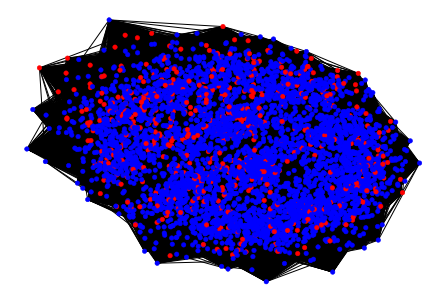
\includegraphics[width=0.7\textwidth]{Moro_network.png}
		\caption{MAG graph of bank telemarketing dataset}
        \label{fig:Moro}
	\end{figure}
  
  \noindent The red dots in figure \ref{fig:Moro} mark the clients which
  decided to invest in the short-term deposit and the blue dots did not invest.
  While this figure masks some of the nodes due to the figure generation
  process, the general pattern becomes apparent. The red nodes appear to be 
  randomly placed in the network which suggests, that the demographic variables 
  which are suitable and were used for the MAG generation process do not
  capture the structure of the label well. The graph further shows, that only a
  relatively small number of clients appear to have invested in the short-term
  deposit. To be more precise, in the dataset only consists of approximately 
  12\% of bank clients which invested in the short-term deposit. The dataset is 
  therefore relatively unbalanced which makes the classification task rather 
  difficult. Graph representation learning using Node2Vec did not provide any 
  useful results and the GNNs also performed rather poorly. In particular, GNNs 
  tendedto classify most clients as non-investors and struggled to accurately
  classify clients which did invest. Due to the unbalanced label data, it was
  loss optimizing to predict most nodes as non-investors rather than learning
  the true observations. Table \ref{table:Moro_conf} shows the confusion matrix
  of the model classifications for the validation data (20\%) using a GraphSage
  GNN.

  \begin{table}[h]
    \centering
    \begin{tabular}{|l|l|c|c}
      \hline
      \diagbox{\textbf{Label}}{\textbf{Predicted}} & \textbf{Did not invest} &
      \textbf{Invested} \\
      \hline
      \textbf{Did not invest} & 1'026 & 30 \\\hline 
      \textbf{Invested} & 119 & 33 \\
      \hline
    \end{tabular}
    \caption{Confusion Matrix Validation Bank Telemarketing Data}
    \label{table:Moro_conf}
  \end{table}


  \noindent The resulting confusion matrix corresponds to an accuracy of
  approximately 87.67\%. The graph generation and subsequent model fitting was
  repeated several times and the accuracies all ranged between 87-90\%. This 
  behavior was observed for both graph based methods and standard machine 
  learning approaches such as ANN or support vector machines (SVM). \\

  \noindent This is part of a larger and common problem in machine learning. 
  Possible remedies might include using loss functions which penalize 
  false classifications harsher than the standard cross entropy loss function
  used for the GNNs. Alternatively one could also reduce the data set by 
  dropping observations such that the remaining dataset is balanced. This 
  approach has its own problem as dropping a large number of observation 
  discards a lot of potentially valuable information. It could also put in 
  question the external validity of the model. These comments point to a 
  separate field of research and could be interesting for a future project. 
  These approaches were not researched in detail and should be taken as 
  suggestions. This thesis will not focus on this problem which is why this 
  issue is not further investigated. \\

  \noindent The failure using graph machine learning methods for this dataset
  reveals, that GNNs are not an easy remedy for unbalanced data. Perhaps if the
  network structure provided clusters which corresponded to the labels, GNNs
  could provide superior results. Given the variables available in the dataset
  and the limitations of using the MAG method, this was not possible. In order
  to check, whether network structure could indeed remedy the unbalanced label
  problem, the label was used for the MAG network generation process. Indeed by
  setting the link-affinity probabilities as follows for the label, superior
  results were achieved:

  \[ \Theta_{label} = 
	\begin{pmatrix}
        0.95 & 0.25 \\
		0.25 & 0.95 \\
	\end{pmatrix}
	\] \\
  
  \noindent The resulting graph when considering the label is shown in figure
  \ref{fig:Moro_bias}.

  \begin{figure}[h]
		\centering
		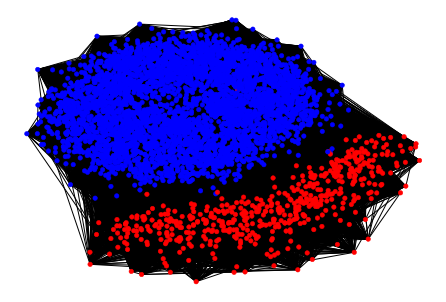
\includegraphics[width=0.7\textwidth]{Moro_network_bias.png}
		\caption{Biased MAG graph of bank telemarketing dataset}
        \label{fig:Moro_bias}
  \end{figure}

  \noindent It now becomes apparent in figure \ref{fig:Moro_bias} that the
  nodes are almost perfectly separated from each other and grouped according to 
  their label. The GNN method GraphSage achieved an accuracy of over 95\% for 
  the graph shown in figure \ref{fig:Moro_bias}. This is of course a form of 
  cheating, as we cannot assume to know the labels of the entire graph and 
  especially when applying the model to new and unseen data which might not 
  contain any label information. It however shows, that if the graph provides 
  node clusters which corresponds to the node labels, that graph machine 
  learning can overcome the problem of unbalanced data to a cerain extent. 
  The difficulty for graph machine learning here is to find graph data including 
  features which naturally captures node clusters which correspond to the node 
  labels. For the synthetic graph generation setting using the MAG model, one 
  would have to collect data which generates clusters via the MAG model that 
  highly correlate with the label. An example for such a dataset was found and 
  while not perfect, it yielded good results and is presented in the following 
  section. 

  \subsection{Airline Passenger Satisfaction Survey}
  
  The US airline passenger satisfaction survey was a survey conducted in 2015
  by J.D. Power and the dataset was retrieved on the website Kaggle
  \citep{JDPower2015,KAGGLE2015}. This dataset revealed to be well suited for
  applying graph machine learning tasks via the MAG method. It further showed
  to be a competitive dataset for classic machine learning methods. Therefore,
  this dataset is suitable for a fair comparison of graph machine learning
  methods vs standard machine learning strategies. This dataset will be
  presented in more detail as it will be used for the detailed analyses which
  are to follow. \\

  \noindent An overview of the US Airline Passenger dataset is shown in table
  \ref{table:airline_summary}. The correlation heatmap of the dataset is
  further shown in figure \ref{fig:corr_heatmap}. The correlation heatmap
  revealed, that the variables "Departure Delay in Minutes" and "Arrival Delay
  in Minutes" are highly correlated. As "Arrival Delay in Minutes" has some
  missing observations, this variable is dropped in favor of "Departure Delay 
  in Minutes". The heatmap and its corresponding correlation matrix reveal,
  that "Gender" is approximately uncorrelated with any of the other variables.
  Further, "Departure Delay in Minutes" appears to be approximately
  uncorrelated with any of the other variables. For that reason, it was tested
  whether both variables could be excluded. The results however revealed, that
  the model performed better if these variables were included in the model. The
  table with a brief description of the variables is provided on the following
  page. The data shown in table \ref{table:airline_summary} and figure
  \ref{fig:corr_heatmap} corresponds to a random sample of 6’000 observations 
  from the training dataset consisting of 103’904 observations.

  \begin{landscape}
  \pagestyle{empty}
  \begin{table}[h]
    \centering
    \begin{tabular}{|l|L|c|c|}
      \hline
      \textbf{Variable} & \textbf{Description} & \textbf{Mean} & \textbf{Range} \\
      \hline
      Gender & Gender of the passengers (Male:0, Female:1) & 0.5076 & 0 - 1
      \\\hline 
      Customer Type & The customer type (loyal customer:0, disloyal customer:1) 
      & 0.18 & 0 - 1 \\\hline
      Age & The actual age of the passengers & 39.101 & 7 - 85 \\\hline
      Type of Travel & Purpose of the flight of the passengers
      (Personal Travel:0, Business Travel:1) & 0.6891 & 0 - 1 \\\hline
      Class & Travel class in the plane of the passengers (Eco:1, Eco Plus:2, 
      Business:3) & - & 0 - 2 \\\hline
      Flight Distance & The flight distance of this journey &
      1'197.438 & 67 - 4'963 \\\hline
      Departure Delay in Minutes & Minutes delayed when departure & 14.808 & 0 - 595 \\\hline
      Arrival Delay in Minutes & Minutes delayed when arrival & 15.159 & 0 -
      589 \\\hline
      Satisfied & Satisfaction: Airline satisfaction level(Satisfied, 
      Neutral or Dissatisfaction) & 0.4295 & 0 - 1 \\\hline
      Inflight WiFi service & Satisfaction level of the inflight WiFi service
      (0:Not Applicable;1-5) & - & 0 - 5 \\\hline
      Ease of Online booking & Satisfaction level of online booking & - & 0 - 5
      \\\hline
      Gate location & Satisfaction level of gate location & - & 0 - 5 \\\hline
      Food and drink & Satisfaction level of Food and drink & - & 0 - 5
      \\\hline
      Online boarding & Satisfaction level of online boarding & - & 0 - 5
      \\\hline
      Seat comfort & Satisfaction level of seat comfort & - & 0 - 5 \\\hline
      Inflight entertainment & Satisfaction level of inflight entertainment & -
                             & 0 - 5 \\\hline
      On-board service & Satisfaction level of on-board service & - & 0 - 5
      \\\hline
      Leg room service & Satisfaction level of leg room service & - & 0 - 5
      \\\hline
      Baggage handling & Satisfaction level of baggage handling & - & 0 - 5
      \\\hline
      Check-in service & Satisfaction level of check-in service & - & 0 - 5
      \\\hline
      Inflight service & Satisfaction level of inflight service & - & 0 - 5
      \\\hline
      Cleanliness & Satisfaction level of cleanliness & - & 0 - 5 \\
      \hline
    \end{tabular}
    \caption{Airline Dataset overview}
    \label{table:airline_summary}
  \end{table}
  \end{landscape}


  \begin{figure}[h]
	  \centering
	  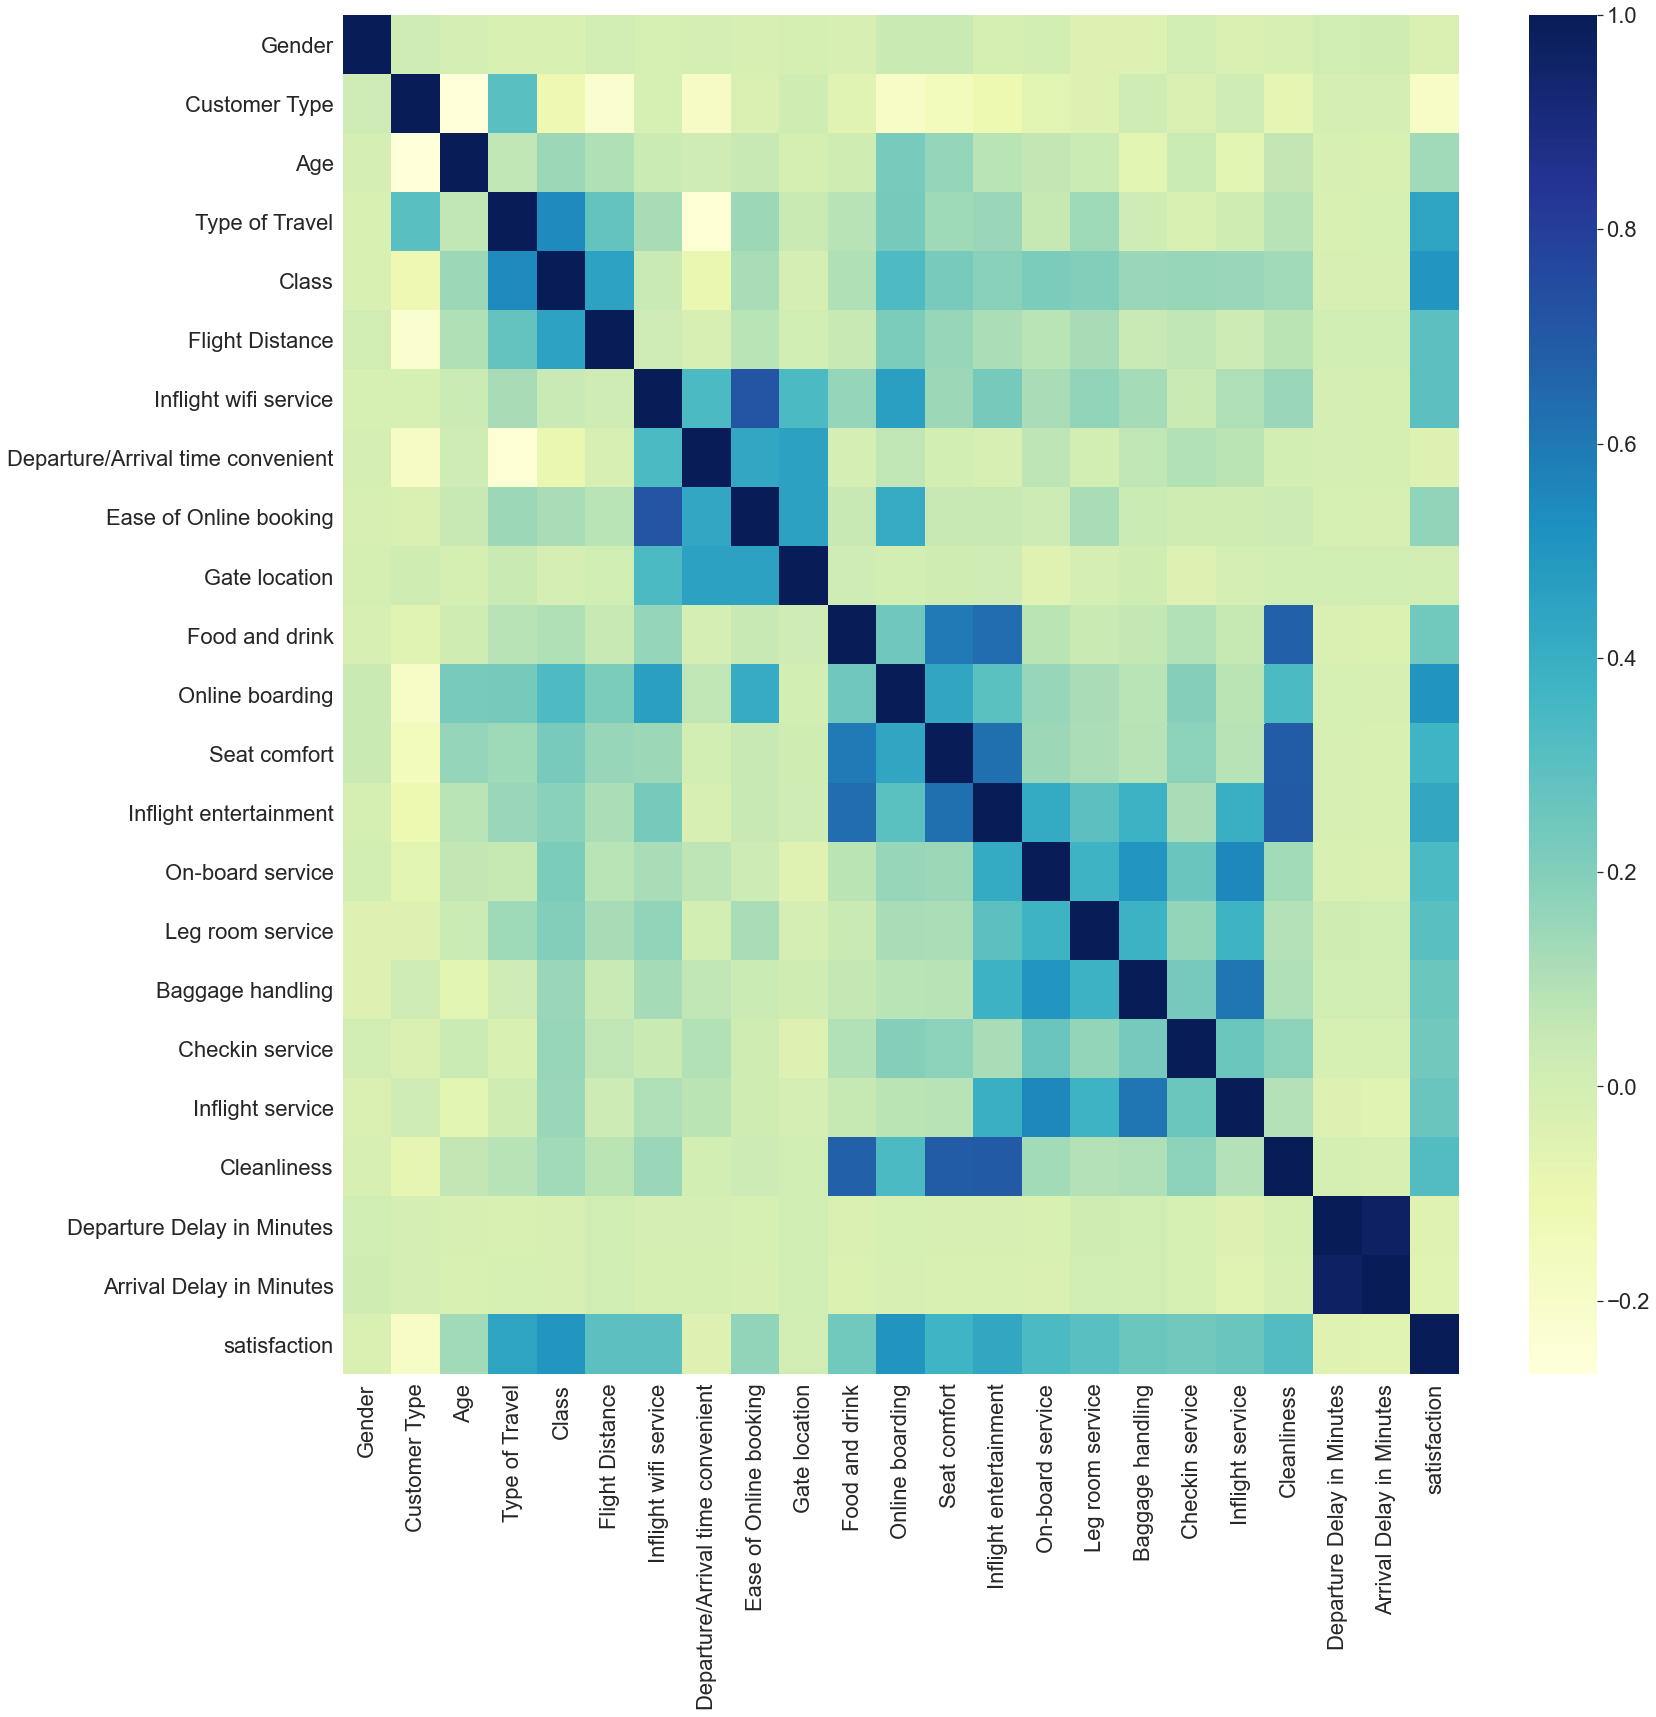
\includegraphics[width=0.8\textwidth]{corr_heatmap.png}
	  \caption{Correlation Heatmap of US Airline Passenger Dataset}
      \label{fig:corr_heatmap}
  \end{figure}

  \noindent The variables of the dataset can further be classified as follows:

  \begin{itemize}
    \item \textbf{Categorical Variables:} Gender, Class, Customer Type, Type of 
      Travel, Satisfaction
    \item \textbf{Ordinal Variables:} Inflight WiFi Service, Ease of Online
      Booking, Gate Location, Food and Drink, Online Boarding, Seat Comfort,
      Inflight Entertainment, On-Board Service, Leg Room Service, Baggage
      Handling, Check-in Service, Inflight Service, Cleanliness
    \item \textbf{Numerical Variables:} Age, Flight Distance, Departure Delay in
      Minutes
  \end{itemize}

  \noindent The categorical variables were dummy coded as shown in table
  \ref{table:airline_summary}. The remaining variables are already correctly
  in the dataset as is. In the following subsection the graph generation
  procedure for the US Airline Passenger dataset is briefly described.

  \subsubsection{Graph Generation}

  To create a graph from the US Airline Passenger Dataset, appropriate
  variables must be selected for the MAG model. The selected variables must be
  of the type such that realistic probabilities can be applied in terms of
  homophily or heterophily. As an example it is for instance difficult to
  assign link-affinity probabilities for people who gave ratings regarding
  the "inflight wifi service". In this case one could assign a probability
  that people who gave high ratings are more similar with relative ease.
  However, does this than also translate to people not liking the wifi-service
  being similar as well? Further, how do we assign probabilities for people who
  are dissimilar? These considerations make the selection of appropriate
  variables for the graph generation more difficult. It is therefore important
  to select variables for which realistic variables for all 3 settings
  which are:

  \begin{itemize}
    \item \textbf{Positively similar observations} (e.g. both observations like 
      the service)
    \item \textbf{Negatively similar observations} (e.g. both observations 
      dislike the service)
    \item \textbf{Dissimilar observations} (Symmetric for undirected graphs, 
      can be asymmetric for directed graphs)
  \end{itemize}
 
  \noindent The variables were selected using the above mentioned 
  considerations. The variables with the corresponding link-affinity 
  probabilities are shown in table \ref{table:link_aff}.

  \begin{table}[h]
    \centering
    \begin{tabular}{|l||L|}
      \hline
      \textbf{Variable Name} & \textbf{Link-Affinity Probabilities}\\
      \hline\hline
      Gender & 0.6, 0.4; 0.4, 0.6  \\\hline 
      Customer Type & 0.8, 0.5; 0.5, 0.8 \\\hline
      Age & 0.90, 0.80, 0.60, 0,40; 0.80, 0.90, 0.80, 0.60; 0.60, 0.80, 0.90,
      0.80; 0.40, 0.60, 0.80, 0.90 \\\hline
      Type of Travel & 0.80, 0.20; 0.20, 0.80 \\\hline
      Class & 0.85, 0.60, 0.45; 0.60, 0.85, 0.60; 0.45, 0.60, 0.85 \\
      \hline
    \end{tabular}
    \caption{Link Affinity Matrices}
    \label{table:link_aff}
  \end{table}

  \noindent The probabilities in table \ref{table:link_aff} correspond to the
  rows of the link-affinity matrices up to the semi-colon. To give a better
  overview, the link-affinity matrix for age is shown explicitly as follows:

  \[ \Theta_{Age} = 
	\begin{pmatrix}
		0.90 & 0.80 & 0.60 & 0.40 \\
        0.80 & 0.90 & 0.80 & 0.60 \\
        0.60 & 0.80 & 0.90 & 0.80 \\
        0.40 & 0.60 & 0.80 & 0.90 \\
	\end{pmatrix}
  \] \\

  \noindent Age was not only selected as an example as its the largest
  link-affinity matrix, it also required some additional data transformation.
  The MAG model can only consider discrete variables which is why age had to be
  binned into categories. Age was binned into 4 bins with 0 if age $<$ 26,
  1 if 26 $\leqslant$ age $<$ 39, 2 if 39 $\leqslant$ age $<$ 50 and 3 if age
  $\geqslant$ 50. The value of the bin corresponds to the position of two
  observations $(u,v)$ in the link-affinity matrix row/column. These bins were
  chosen according to the interquartile lengths present in the variable age. \\

  \noindent For assigning probabilities there exist no rules as to how these
  must be applied. The paper by \cite{kim2012multiplicative} shows the 4 common
  structures of homophily, heterophily, core-periphery and random for creating
  graphs. For this thesis, the homophily approach was selected where the more
  similar two observations are, the more likely they are to form a connection.
  For the selected variables reasonable similarity and dissimilarity 
  probabilities could be assigned in a homophily setting. The probabilities were
  assigned based on personal intuition and experimentation. Several graphs were
  created with different probabilities and the probabilities shown in table
  \ref{table:link_aff} appear to generate reasonable graphs. There is however
  no exact science or selection criteria applied when choosing the
  probabilities. \\

  \noindent A random sub-sample of 6'000 observations was retrieved from the
  training dataset consisting of 103’904 observations. With this random
  sub-sample the adjacency matrix for the resulting graph was generated using
  algorithm \ref{algo:MAG} with the link-affinity matrices shown in table
  \ref{table:link_aff}. The random sub-sample was retrieved due to the
  computational cost involved applying algorithm \ref{algo:MAG}. Simulations
  involving creating graphs with different random sub-samples suggest, that the
  random sub-samples are representative for the entire dataset. The resulting
  graph used for the subsequent analyses is shown in figure
  \ref{fig:us_airline_graph}.

  \begin{figure}[h]
	  \centering
	  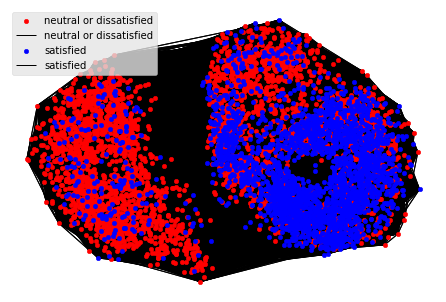
\includegraphics[width=0.7\textwidth]{us_airline_graph.png}
	  \caption{Graph of US Airline Passenger Dataset}
      \label{fig:us_airline_graph}
  \end{figure}
  
  \noindent The network shown in figure \ref{fig:us_airline_graph} show the
  emergence of two groups. In addition one can see, that most satisfied airline
  passengers appear to be somewhat clustered together. To gain a deeper
  understanding of the dynamics involved in the network formation, the nodes of
  the network (excluding the edges) are plotted in figure
  \ref{fig:us_airline_nodes}.

  \begin{figure}[h]
	  \centering
	  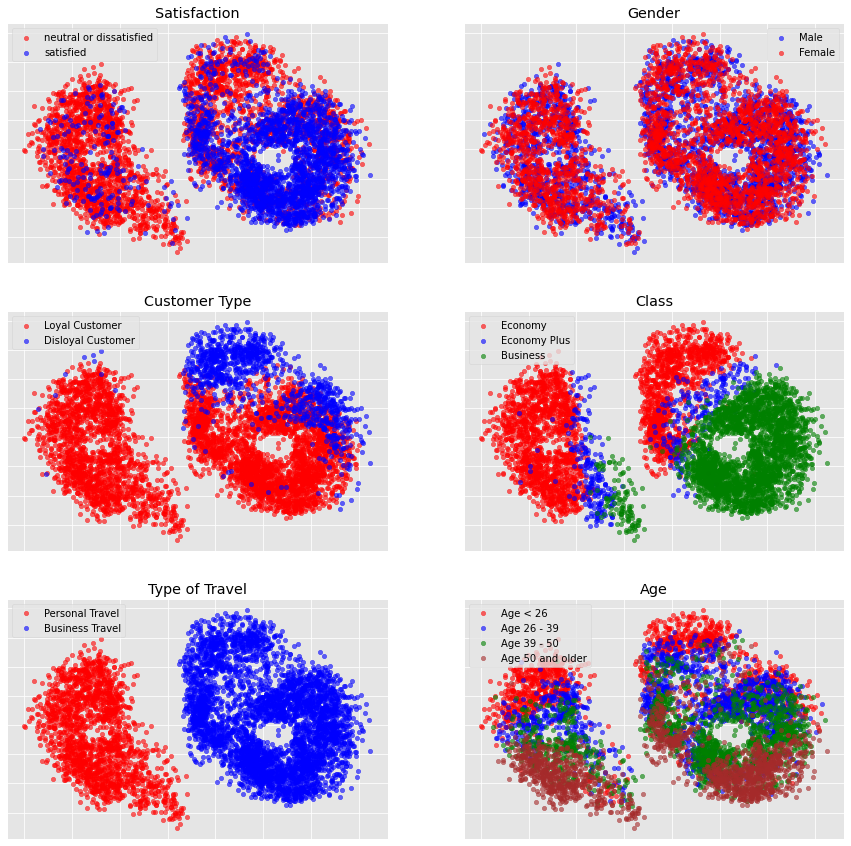
\includegraphics[width=0.8\textwidth]{us_airline_nodes.png}
	  \caption{Graph Nodes of US Airline Passenger Dataset}
      \label{fig:us_airline_nodes}
  \end{figure}

  \noindent Figure \ref{fig:us_airline_nodes} plots the nodes of the network
  for the label "Satisfaction" and the 5 variables used for the graph
  generation. The nodes were plotted with $\alpha = 0.6$ to avoid covering
  nodes during the graph generation process. The node plots reveal interesting
  relationships. First, we can see that people traveling for business purposes
  tend to be more satisfied than people traveling for personal reasons. On a
  second level we can see, that people who flew business class appear to be
  mostly satisfied and constitute the majority of the cluster with satisfied
  passengers visible on figures \ref{fig:us_airline_graph} \&
  \ref{fig:us_airline_nodes}. When comparing to people traveling for personal
  reasons, "Class" does not appear to be a determining factor for satisfaction.
  For the variable "Age" we can see that older people tend to fly more business
  class when on a business trip. In addition, older people traveling for
  business purposes tend to be loyal customers compared to younger customers.
  Interestingly, these relationships do appear to be present for passengers
  traveling for personal reasons. Interestingly, most passenger traveling for
  personal reasons appear to be loyal customers. This however does not appear
  to translate into positive satisfaction. Lastly, the variable Gender does not
  appear to form any distinguishable clusters. For that reason it was
  considered to omit this variable for the graph generation process. This was
  tested and the resulting graph yielded similar structures within the graph.
  The graph was however more spread out and neighborhood structures were less
  clear. In addition, the graph without gender did not perform as well in the
  subsequent ML tasks. For those reasons, gender was kept for the graph
  generation process. \\

  \noindent Last but not least, the graph is described using metrics from graph
  theory. The degree distribution as well as the distributions of the 
  centrality measures eigenvector centrality, closeness centrality and 
  betweenness centrality are shown in figure \ref{fig:centrality_measures}.

  \begin{figure}[h]
	  \centering
	  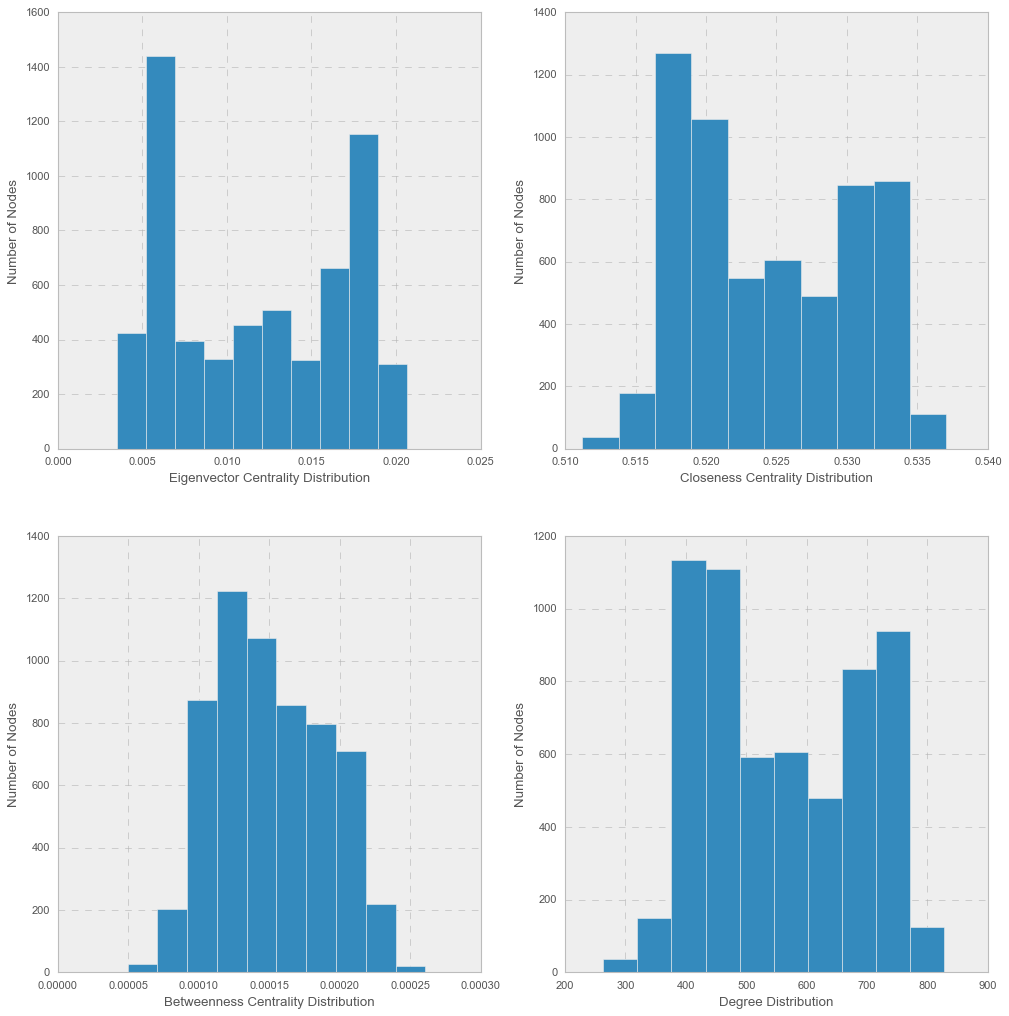
\includegraphics[width=0.7\textwidth]{centrality_measures.png}
	  \caption{Graph Statistics}
      \label{fig:centrality_measures}
  \end{figure}

  \noindent The network further has a density of approximately 0.0933. This
  means that 9\% of the maximum number of connections formed in the network.
  Nevertheless when looking at the degree distribution histogram we can see 
  that a all nodes have a large number of connections ranging between 263 -
  828 with an average of 559.63 connections. Further, the distribution has two
  modes. The eigenvector centrality distribution shows, that all nodes have a
  very low centrality measure and therefore none of the nodes appear to have a
  large impact in terms of eigenvector centrality. The closeness centrality
  distribution shows, that all nodes have an average closeness centrality
  ranging from 0.51 - 0.53. This means that every node is similarly connected
  and has an average impact for disseminating information across the network.
  Lastly, the betweenness centrality distribution reveals that there are no
  bottle-necks through which information flows. \\

  \noindent As a reference point, it is important to compare the properties of
  the created graph to real world graphs. In our case, the most appropriate for
  comparison is a social network. Common structures of social networks are
  \citep{watts1998collective,newman2006structure,Newman2010,
  kim2012multiplicative}:

  \begin{enumerate}
    \item Degree distributions typically follow a power law distribution
    \item Emergence of a giant connected component
    \item Core-periphery structure
  \end{enumerate}

  \noindent This power law degree distribution and emergence of a giant
  connected component creates network structures that have an onion
  (core-periphery) structure \citep[p. 121]{kim2012multiplicative}. This
  indicates, that most social networks have a few very highly connected nodes
  and many nodes with few connections. This creates a right skewed degree 
  distribution which also lead to a right skewed eigenvector centrality and
  closeness centrality distribution. For the betweenness centrality, we would
  also expect, that more central nodes in a core-periphery network structure
  would exhibit some bottle-neck properties for the central nodes. For that
  reason we would expect central nodes to have a higher betweenness centrality.
  When we look at the distributions in figure \ref{fig:centrality_measures}
  this does not correspond to the power law degree distribution and the effect
  this has on the centrality measures observed in real social networks. This
  indicates, that the graph created with the MAG method does not share the
  properties ovserved in real graphs. In order to generate a graph which
  shares the properties of real graphs, one would have to adapt the 
  link-affinity properties to the core-periphery setting as shown in figure
  \ref{fig:link-affinity}. Forcing this core-periphery structure is however not
  purposeful for this thesis. Further, the aim of this thesis is not
  necessarily to create realistic graphs rather than to create useful graphs 
  for graph machine learning. The results revealed that the graph is indeed
  useful for graph machine learining. In addition, limiting factors of the
  graph were discovered. These aspects will be discussed further in the results
  and discussion section. 


  \subsection{Stochastic vs. Deterministic MAG}

  As addressed in section \ref{section:self_survey}, the question was raised 
  as to whether the MAG should form connections between observations
  stochastically or whether a deterministic setting yields better results. The 
  first insight gained when investigating this question lies in the fact that 
  the probability of two observations is generally very low. When setting the 
  threshold to 0.5, not a single connection between observations was made. This
  makes sense as the probability of a connection being formed decreases by
  design as the number of generation variables increases. This is implicitly
  shown in equation \ref{eq:MAG} where the product of probabilities is bound to
  decrease. For this reason, it is suggested to set $K=\rho\log_{2}N$
  for some constant $\rho$ \citep[p. 122]{kim2012multiplicative}. For the
  purpose of this thesis, the generation variables were selected such that
  $K\leqslant\log_{2} N$. The airline passenger satisfaction survey was used
  for a deterministic graph generation. The threshold probability for a
  connection was set to 0.2 in the MAG model. The resulting graph consisted of
  several disconnected sub-graphs which were for the most part clustered
  according to their group membership. Figure \ref{fig:det_MAG} shows the
  respective plots of the graph generation variables where the edge connections
  were removed. The sub-graphs are unfortunately small, however all graphs
  combined include all 6'000 nodes. The plots are meant to provide a high-level
  overview of the clusters in the sub-plots. 

  \begin{figure}[h]
		\centering
		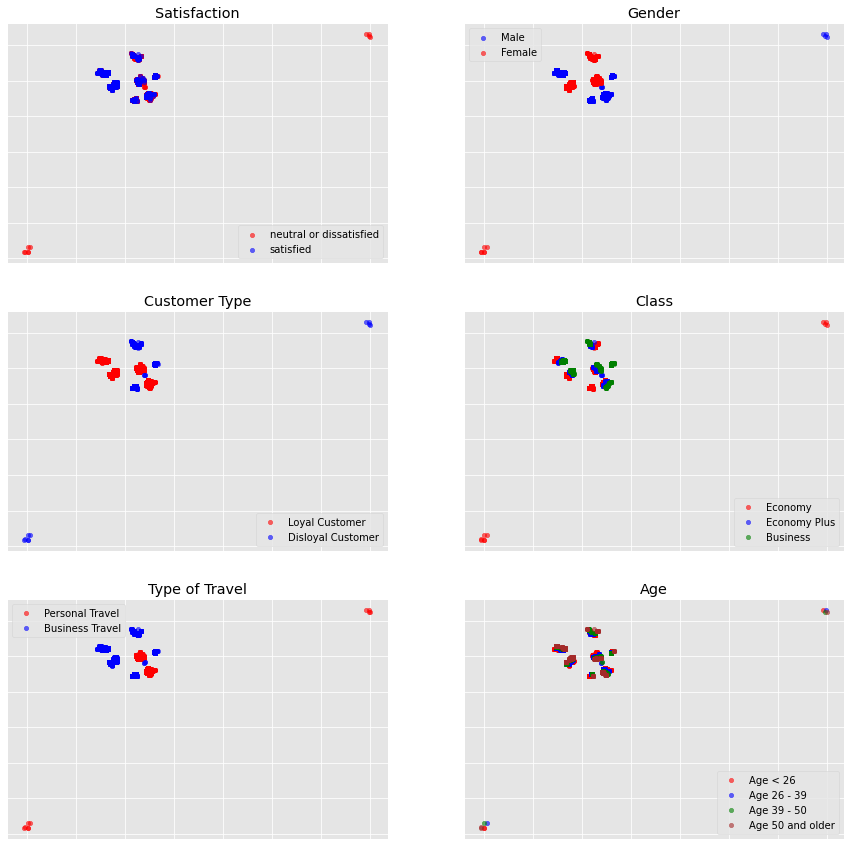
\includegraphics[width=0.7\textwidth]{deterministic_MAG.png}
		\caption{Deterministic MAG graph}
        \label{fig:det_MAG}
  \end{figure}

  \noindent In short, the deterministic graph clustering creates disconnected 
  sub-graphs which forms clusters based on the nodes similarity to each other.
  In terms of performance, the performance and loss behavior of both the
  deterministically and stochastically generated graphs are virtually
  identical. This was true for the datasets considered for this thesis. For the 
  purpose of visualization the stochastically generated graph appears
  to be more useful, as one can identify the different cluster on a single
  connected graph.  For this reason, the stochastic graph generation process is 
  kept. Nevertheless, deterministic graph generation appears to be useful if 
  one wants to separate nodes in to more homogeneous sub-graphs. These 
  sub-graphs or clusters could then be used for subsequent machine learning 
  tasks with a cluster specific target. The clusters further could reveal 
  information as to which clusters tend to be more or less satisfied. This is 
  an area which could be interesting for future research. It is however not 
  the focus of this thesis which is why it is not further investigated. 
  
